\chapter{Nawigacje dla rowerzystów}
\label{cha:nawigacje_dla_rowerzystow}

\section{Specyfika tematu}

Nawigacja jako ogólne zagadnienie funkcjonuje w świadomości ludzi już od dłuższego czasu. Wprawdzie jeszcze 20-25 lat temu mało kto wyobrażał sobie jazdę samochodem po nieznanych terenach bez wcześniejszego zaplanowania trasy przy pomocy papierowej mapy, to jednak ostatnia dekada przyniosła w zasadzie całkowite wyparcie takiego stanu rzeczy. Odpowiadają za to właśnie nawigacje, najpierw jako autonomiczne urządzenia, potem jako aplikacje na smartfony (choć te pierwsze nadal funkcjonują na rynku i mają się całkiem dobrze). Tak duży staż rynkowy danego rozwiązania daje podstawy do stwierdzenia, że wszystko co istotne zostało już w tej materii wymyślone i zaimplementowane. Być może jest to prawda, a być może czeka nas jeszcze niejedna rewolucja (z gatunku raczej tych nie zauważalnych przez przeciętnego użytkownika), co nie zmienia jednak faktu, że fundamenty są i zapewne pozostaną te same. Nawigacje bowiem w dużej mierze opierają swe działanie na poprawności czterech głównych czynników:
\begin{itemize}
\item dokładnych i aktualnych danych o infrastrukturze 
\item zbudowania grafu relacji powyższych danych
\item możliwie jak najbardziej efektywnego i optymalnego algorytmu do wyszukiwania najkrótszej ścieżki w tymże grafie
\item przejrzystej i intuicyjnej wizualizacji wyników
\end{itemize}
I tak jak ostatni punkt, to w dużej mierze kwestia estetyki (choć oczywiście nie tylko), tak pierwsze trzy diametralnie wpływają na jakość wskazań. W przypadku konkretnie nawigacji rowerowych największą trudnością jest punkt pierwszy. Prawidłowe dane na temat ścieżek rowerowych, czy też dróg przyjaznych rowerzystom, to towar mocno deficytowy. Jednakże nawet jego posiadanie nie gwarantuje pełni sukcesu, gdyż tematyka infrastruktury rowerowej jest znacznie bardziej złożona aniżeli infrastruktury samochodowej. W tym drugim przypadku działa prosty warunek: jest droga znaczy da się przejechać. Oczywiście należy także uwzględnić chociażby kierunkowość ulic, jednak na tym poziom komplikacji się w zasadzie kończy. Z rowerem sprawa wygląda inaczej, gdyż czasami bardzo trudno jest jednoznacznie określić wszystkie miejsca, przez które da się oraz można przejechać rowerem. Przeszkodą mogą być zwykłe schody, czy też samo-zamykająca się brama, bądź szlaban. Działa to także w drugą stronę: dwie sąsiadujące ze sobą lokalne uliczki mogą nie być połączone w rozumieniu samochodowym, a jednak dzielić je może jedynie pas betonowych donic na kwiaty lub słupki. Przykłady można by mnożyć bez końca, niemożliwym jest uwzględnienie absolutnie każdej realnie możliwej relacji, zwłaszcza w przypadku większej skali, jak obszar całego państwa. W mniejszym zakresie – jak rozpiętość średniej wielkości miasta, jakim jest Kraków – jest to w większym lub mniejszym stopniu wykonalne, choć z pewnością niełatwe i wymagające wielu testów praktycznych wykonanych bezpośrednio w terenie. Podobnym problemem jest kwalifikacja zwykłych dróg, na te przyjazne rowerom oraz te nieprzyjazne. Wprawdzie dylemat ten, w przypadku niniejszej aplikacji, został niejako rozwiązany przez osoby trzecie, gdyż ZIKiT sam dostarcza również dane o preferowanych ulicach do użytku także rowerowego, to jednak nie da się ukryć pewnego drobnego paradoksu z tym związanego. Otóż ulice przyjazne rowerzyście powinny charakteryzować się możliwie jak najniższą prędkością maksymalną zdefiniowaną dla pojazdów mechanicznych oraz relatywnie małym natężeniem ruchu tychże. Takie ulice to zazwyczaj lokalne drogi osiedlowe, których przecież jedynym celem jest doprowadzenie ruchu do większych arterii, a te już przyjazne rowerzyście z pewnością nie są. Oczywiście można mieć nadzieje, że każda większa trasa komunikacyjna będzie posiadać równoległą do siebie ścieżką rowerową, ale niestety w Krakowie na ten moment nie ma to jeszcze miejsca.\newline
Warto się także pochylić nad wspomnianą wcześniej bazą danych ZIKiTu odnoszącą się do dróg przyjaznych rowerzyście. Zostały one zdefiniowane jako tzw. drogi tempo 30, czyli takie na których obowiązuje ograniczenie prędkości do 30 km/h. Bardzo trudno o rzetelny osąd takiego, a nie innego wyboru. Prawdopodobnie wynikało to z chęci stworzenia jak najbardziej kompletnej sieci możliwych dróg.Gdzie konkretnie zdefiniowane zostały strefy z tego typu drogami można zobaczyć na mapie wizualizacji dancyh ZIKiTu (Rys. 3.1.).\newline

\begin{figure}[H]
\centering
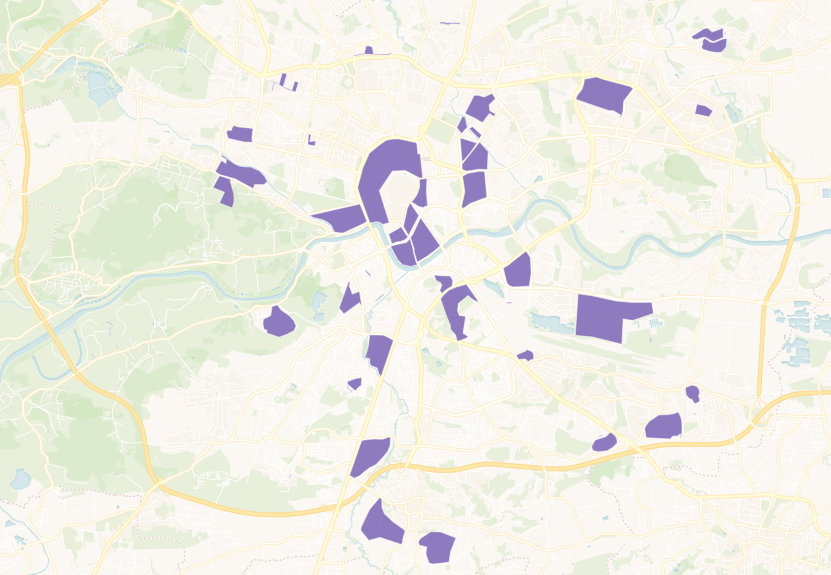
\includegraphics[width=\textwidth]{tempo30}
\caption{Strefy tzw. ulic tempo 30; źródło ZIKiT: \protect\url{https://zikit.carto.com/tables/tempo30krakow/public\#/map} (stan na dzień 6.09.2019).}
\end{figure}

Kwestia poprawnego grafu relacji to także trudny temat. Samo jego zbudowanie to jedno, wielokroć istotniejszą sprawą w kontekście nawigacji rowerowej jest waga danych ścieżek. Chodzi oczywiście o – nierzadką przecież – sytuację, gdy w dane miejsce prowadzą zarówno autonomiczne ścieżki rowerowe (rozdzielone od jezdni), te wyznaczone w torze jezdni samochodowej oraz drogi z kategorii przyjaznych rowerzyście. W jaki sposób odpowiednio dobrać wagi? Co całkowicie zrozumiałe nie mogą być one równoważne, gdyż wtedy dochodziłoby do absurdalnych sytuacji, gdy nawigacja prowadziłaby po samych drogach samochodowych tylko dlatego, że trasa po autonomicznej ścieżce rowerowa byłaby dłuższa, dajmy na to, dosłownie o parę metrów. Wagi te nie mogą być także zbyt zróżnicowane, gdyż wtedy dochodziłoby do sytuacji odwrotnych: nawigacja sugerowałaby wprawdzie trasę po samych autonomicznych ścieżkach rowerowych, ale znacznie dłuższą, niż gdyby skorzystać w paru miejscach ze „skrótu” w postaci drogi lokalnej. Stąd tak ważne jest by autorzy takiej nawigacji dobrze znali obszar ( w tym przypadku miasto Kraków), po którym ma ona prowadzić. Bez praktycznej znajomości topografii, mogłoby być ciężko wykryć pewne błędy w postaci nielogicznych tras.

\section{Istniejące rozwiązania}

Światowy rynek nawigacji rowerowych nie grzeszy obfitością, nie mówiąc już o rozwiązaniach stricte dla terenów Polski. Oczywiście funkcjonują rozwiązania gigantów jak choćby Mapy Google (zarówno wersja webowa jak i na urządzenia mobilne), czy Mapy Apple (wyłącznie na urządzenie mobilne), jednak ich główną domeną jest nawigacja przygotowana dla samochodów, odmiana dla rowerzystów, to raczej dodatek traktowany obecnie nieco po macoszemu i oparty na nie do końca sprawdzonych danych, co wyraźnie widać w ich działaniu. Dlatego też rozwiązania te wpadają w proste pułapki jak na przykład wyznaczanie trasy przez schody bądź pomijanie tzw. kontrapasów rowerowych. Nie ma się jednak temu co dziwić, jeśli weźmiemy pod uwagę ogrom obszaru jaki obejmują niniejsze projekty. Niemałym problemem w ich przypadku jest również mocne opóźnienie aktualizacji w stosunku do rzeczywistych zmian w infrastrukturze. Istnieją oczywiście również profesjonalne urządzenia nazywane „nawigacją rowerową”, jednak są to produkty dość drogie i skierowane raczej do co najmniej średnio-zaawansowanych rowerzystów, a nie do człowieka, który po prostu chce dostać się do pracy przy pomocy rowery. Inną sprawą jest, ze tego typu profesjonalne nawigacje starają się za wszelką cenę unikać zatłoczonych tras i większych miast, siłą rzeczy więc nie nadają się do nawigowania po metropoliach. \newline
Osobnym przypadkiem jest aplikacja Bike Citizens, dostępna zarówno w formie webowej jak i na urządzenia mobilne. U podstaw tego niemieckiego projektu leży wyznaczanie trasy dla rowerzystów, co zresztą sugeruje już jej angielska nazwa. Co więcej, swoje działanie ogranicza jedynie do wybranych europejskich miast (obecnie jest ich około 450), co pozwala mieć nadzieję na poprawniejsze wyniki niż masowe rozwiązania. I faktycznie, choć Bike Citizens korzysta z danych OpenStreetMap, to jednak mocno je modyfikuje dzięki czemu, są całkiem obszerne i precyzyjne. Efektem tego aplikacji zdarza się wyznaczać trasy znacznie lepsze niż opisywane wyżej rozwiązania informatycznych gigantów. Niestety kluczowym jest sformułowanie „zdarza się”. Bike Citizens zbyt często popełnia błędy projektów o zbyt dużej skali, największe problemy mając z odpowiednim dopasowaniem wag, co skutkuje nazbyt nadgorliwym prowadzeniem po ścieżkach rowerowych (przez co trasa potrafi być przesadnie długa). Jej dużą wadą jest też oparcie się o OpenStreetMap. Wprawdzie jej dane są zazwyczaj bardzo aktualne, a dodatkowo Bike Citizens samo je jeszcze poprawia (z różnym skutkiem z powodu – jak zostało napisane wyżej – zbyt dużej skali), to jednak fakt tworzenia ich przez zwykłych użytkowników, a nie ludzi obeznanych z tematem, ma kilka niekorzystnych następstw. Po pierwsze dane potrafią być bardzo niespójne. Istnieje także ryzyko dużych przekłamań względem rzeczywistości, czy po prostu próby nieśmiesznego żartu w postaci wprowadzenia celowo zupełnie bezsensownych danych. Wprawdzie takie odchyłki zostają szybko wyłapywane i poprawiane, jednak stwierdzenie „szybko” może oznaczać nawet parę dni, w trakcie których ktoś może się bardzo zdziwić wyznaczając trasę przy pomocy aplikacji.\newline
Istnieją jeszcze pojedyncze projekty, które starają się nawigować rowerzystów (lub choćby wyznaczać dla nich trasę) jak Mapa Polski, naviki czy Locus Mapa. Jednak wszystkie te rozwiązania bazują na którymś z wyżej wymienionych projektów, nie dokładając wiele od siebie, a często oferując gorsze algorytmy wyszukiwania, czy mniej intuicyjny interfejs. 
